\documentclass[11pt, a4paper]{article}

%\usepackage[T1]{fontenc}
%\usepackage{fullpage}

\usepackage[utf8]{inputenc} % comment when using lualatex
\usepackage[italian]{babel} % lingua e a-capo-sillabato
\usepackage{graphicx}
\usepackage[hidelinks]{hyperref} % link di pagina
\usepackage[bottom]{footmisc} % note appiccicate al fondo della pagina
\usepackage{float} % per posizionamento immagini
\usepackage{amsthm} % per ambienti stile teorema
\usepackage{tabularx} %tabelle
\usepackage[table]{xcolor} %colore caselle
\usepackage{enumitem} %additional commands for lists
\usepackage{fancyhdr}
\usepackage[font=footnotesize,labelfont=bf]{caption} % small caption font-size



\pagestyle{fancy}
\fancyhf{}% Clear header/footer
\fancyfoot[C]{\thepage} %add page number
\fancyhead[C]{\footnotesize\textit{Documento:} D3 \hfill SleepCode \hfill \textit{Versione:} 1.0}
\renewcommand{\headrule}{{\color{red!70}\rule{\textwidth}{2pt}}}
\setlength{\headheight}{22pt}

\renewcommand\UrlFont{\color{blue}\rmfamily} % colore link

\theoremstyle{definition} % stile dei newtheorem (non italizzati)
\newtheorem{funcreq}{RF} %% numerazione dei requisiti funzionali
\newtheorem{nonfuncreq}{RNF} %% requisiti non funzionali
\newtheorem{backend}{BE}
\newtheorem{frontend}{FE}




\title{Documento di Architettura}

\author{Raffaele \textsc{Castagna}\\
Alberto \textsc{Rovesti}\\
Zeno \textsc{Saletti}}

\newcommand{\groupNumber}{G17}

% Web address for the project (if any)
% \newcommand{\homepage}{\url{https://www.}}

% data
\date{\today}

\makeatletter{}

\newcommand\blfootnote[1]{%
  \begingroup
  \renewcommand\thefootnote{}\footnote{#1}%
  \addtocounter{footnote}{-1}%
  \endgroup
}

% IL PREAMBOLO FINISCE QUI %%%%%%%%%%%%%%%%%%%%%%%%%%%%%%%%%%%%%%%%%%%%%%%%%%%%



\begin{document}

% La pagina di copertina si trova in un file .tex a parte
% NON MODIFICARE QUESTO COMANDO!!!
\begin{titlepage}
\newcommand{\HRule}{\rule{\linewidth}{0.3mm}} % Defines a new command for horizontal lines, change thickness here
\center % Centre everything on the page

%------------------------------------------------
%	Logo
%------------------------------------------------

\includegraphics[width=0.3\textwidth]{materiale/UniTrento_logo_ITA_colore.png}\\[0.5cm]
%------------------------------------------------
%	Headings
%------------------------------------------------
\textsc{\Large Dipartimento di Ingegneria\\e Scienza dell'Informazione}\\[1.5cm]

{\Huge\textbf{Sleep Code}}\\[0.5cm]
\textsc{\large Progetto per il Corso di Ingegneria del Software}\\
\textsc{\large Anno Accademico 2023-2024}\\[0.5cm]

%------------------------------------------------
%	Title
%------------------------------------------------

\HRule\\[0.4cm]
{\huge\bfseries \@title}\\[0.1cm]
\HRule\\[1cm]

\begin{minipage}{\textwidth}
\begin{flushleft}
\textit{Descrizione:} documento di analisi dei requisiti funzionali, non funzionali, front-end e back-end.
\end{flushleft}
\end{minipage}\\[1.5cm]


\begin{minipage}{0.4\textwidth}
\begin{flushleft}
\large
\textit{Numero documento:} D1
\end{flushleft}
\end{minipage}
\begin{minipage}{0.4\textwidth}
\begin{flushright}
\large
\textit{Versione documento:} 2.4
\end{flushright}
\end{minipage}\\[1.5cm]

%------------------------------------------------
%	Author(s)
%------------------------------------------------
\begin{minipage}{0.4\textwidth}
\begin{flushleft}
\large
\textit{Membri del gruppo:}\\
\@author % Your name
\end{flushleft}
\end{minipage}
~
\begin{minipage}{0.4\textwidth}
\begin{flushright}
\large
\textit{Numero gruppo: }
\groupNumber
\end{flushright}
\end{minipage}

% 	If you don't want a supervisor, uncomment the two lines below and comment the code above
% 	{\large\textit{Author(s)}}\\
% 	\@author % Your name

%------------------------------------------------
%	Date
%------------------------------------------------

\vfill\vfill
\textit{Ultima revisione:}
{\@date}

\end{titlepage}

\tableofcontents\blfootnote{\textbf{Consigli utili per la consultazione del testo:} Se il lettore per file \texttt{.pdf} attualmente in uso lo consente, è possible navigare con più semplicità e velocità all'interno di questo documento cliccando sugli elementi dell'indice.}

\newpage

\section*{Scopo del documento}
In questo documento viene riportata la definizione dell'architettura del
progetto \textit{SleepCode} impiegando diagrammi delle classi, realizzati
secondo gli standard di Unified Modeling Language (UML), e codice scritto in Object
Constraint Language (OCL). Nel documento precedente (D2, \textit{Specifica
dei Requisiti}) sono stati presentati il diagramma degli use case, quello
di contesto e infine il Diagramma dei Componenti. Considerando tale
progettazione, viene ora definita l'architettura del sistema specificando
in modo più dettagliato le classi che dovranno essere implementate sotto forma di
codice, insieme alla logica che regola il comportamento del software che
si intende realizzare.

Il linguaggio UML, utilizzato per descrivere le classi, è supportato da
codice OCL, impiegato invece per catturare gli aspetti logici citati sopra,
che non sarebbero altrimenti esprimibili formalmente mediante i soli diagrammi delle
classi.


\newpage
\section{Definizione delle classi}
Nella presente sezione vengono illustrate in linguaggio UML le classi
previste dal progetto \textit{SleepCode}. Ogni componente del diagramma
dei componenti, presente nel documento D2, viene qui rappresentato
in forma di una o più classi. Le classi individuate sono costituite
da un nome, un insieme di attributi che identificano i dati gestiti dalla
classe stessa e una lista di metodi che definiscono le operazioni
eseguibili da quella classe. Eventuali relazioni tra classi sono evidenziate
da alcune associazioni.

\subsection{Utenti}
L'attore che nel diagramma di contesto usufruisce delle funzionalità offerte
dal sistema è l'utente. Come descritto nei documenti di Analisi (D1) e
e Specifica dei Requisiti (D2), esistono tre categorie di utenti: anonimo, autenticato
e amministratore. La Figura \ref{utenti} illustra le rispettive classi.

\begin{figure}[H]
\centering
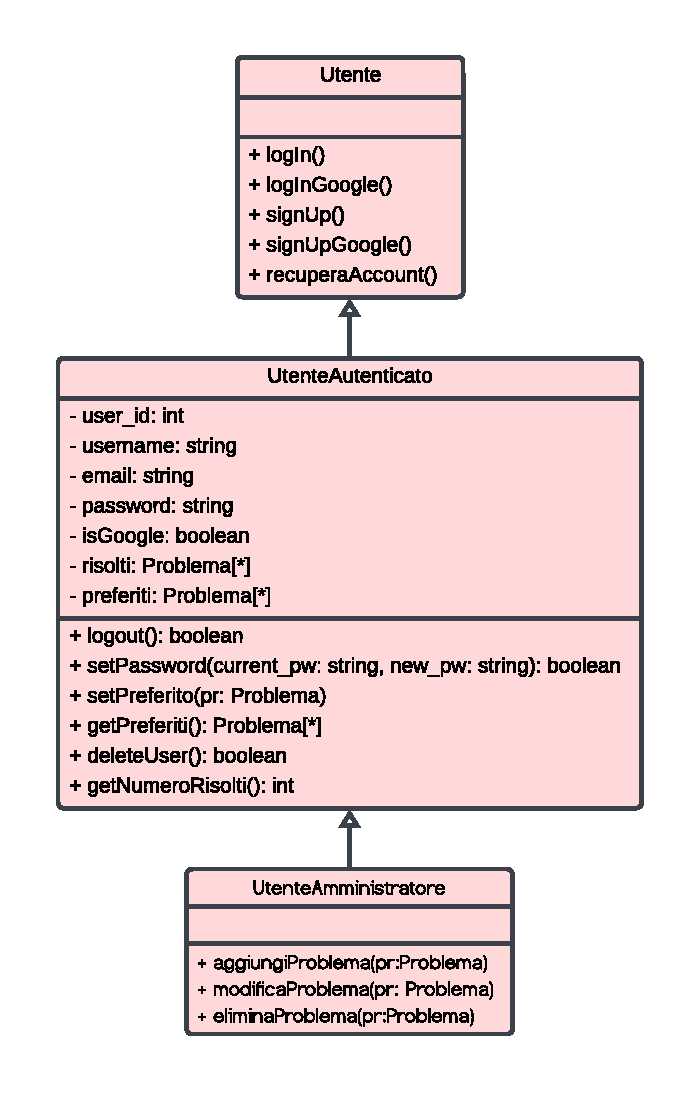
\includegraphics[scale = 0.71]{materiale/class-utenti.pdf}
\caption{Definizione della classe \texttt{Utente} e delle sue generalizzazioni}
\label{utenti}
\end{figure}

Dal momento che tutte queste categorie condividono alcune funzionalità, è stata
creata una classe \texttt{Utente}, che logicamente corrisponde alla categoria
degli utenti anonimi, ovvero utenti che non hanno effettuato il login. Di fatto,
non è prevista la memorizzazione di alcuna informazione riguardo a questa categoria
di utenti e le uniche operazioni disponibili sono:
\begin{itemize}
    \item \texttt{login()}: richiesta di accesso con sistema di credenziali interne.
    \item \texttt{signUp()}: richiesta di registrazione con sistema di credenziali interne.
    \item \texttt{loginGoogle(), signUpGoogle()}: controparti dei metodi precedenti, che
    però si avvalgono dei servizi di autenticazione Google.

    \item \texttt{recuperaAccount()}: richiesta di avvio della procedura di recupero account.
\end{itemize}
Da questa prima classe viene definita, mediante generalizzazione, la classe
\texttt{UtenteAutenticato}, che aggiunge metodi e attributi accessibili previo
login:
\begin{itemize}
    \item \texttt{user\_id}: dal momento che email e password dell'account di sistema
    possono essere modificate dall'utente autenticato, la classe contiene questo
    attributo con ruolo di identificatore univoco.

    \item \texttt{username, email, password}: i dati richiesti per creare un
    account. In caso di autenticazione con Google, è richiesto che la classe
    memorizzi solo l'indirizzo email impiegato e l'username.

    \item \texttt{isGoogle}: parametro che distingue gli account collegati con
    Google da account registrati con il meccanismo di credenziali interne.

    \item \texttt{risolti[*]}: insieme dei problemi risolti dall'utente.

    \item \texttt{preferiti[*]}: insieme dei problemi preferiti dell'utente.

    \item \texttt{logout()}: richiesta di logout.
    
    \item \texttt{setEmail, setPassword}: procedure utili a modificare le credenziali
    dell'account. Oltre alle nuove credenziali, viene richiesta, per questioni di sicurezza,
    la password attualmente in uso. Entrambi i metodi restituiscono una risposta
    di tipo booleana per segnalare il successo o l'insuccesso delle rispettive operazioni.

    \item \texttt{setPreferito}: questo metodo provvede ad aggiungere o
    eliminare dalla lista dei preferiti dell'utente il problema fornito: se
    presente, esso viene rimosso dalla lista, altrimenti viene aggiunto.

    \item \texttt{getPreferiti}: i preferiti dell'utente autenticato vengono
    messi a diposizione all'esterno della classe grazie a questo metodo.
    Come descritto nel diagramma dei componenti, in questo modo viene
    realizzata l'interfaccia che passa i preferiti dell'utente dal Gestore
    Utente verso il Catalogo, in modo da visualizzarli nella lista dei
    problemi.
\end{itemize}
Infine, un'ulteriore generalizzazione specifica le funzionalità aggiuntive
dell'utente amministratore, ovvero metodi utili alla gestione del catalogo
e dei problemi:
\texttt{aggiungiProblema}, \texttt{modificaProblema}, \texttt{eliminaProblema}.


Facendo riferimento al Diagramma dei Componenti del
documento D2, queste classi sono state in parte estratte da tre componenti
distinti che si occupano dell'interazione con l'utente esterno: dalla
\textit{Pagina di Autenticazione} sono stati raggruppate le interfacce che
si trovano in \texttt{Utente}; in \texttt{UtenteAutenticato} sono state
raccolte le interfacce presenti nel componente \textit{Gestore Utente};
in \texttt{UtenteAmministratore} sono state raggruppate alcune delle interfacce
definite nel componente \textit{Catalogo}.






\newpage
\subsection{Gestione autenticazione}
Nel diagramma di contesto, l'autenticazione si avvale di due sistemi
subordinati: \textit{Firebase}, che si occupa di memorizzare gli account
registrati con sistema di autenticazione interno, e \textit{Google SignIn},
con il quale è possibile effettuare la registrazione o l'autenticazione
mediante un account Google.

Il componente \textit{Gestore Autenticazione} del rispettivo diagramma si
occupa di interagire con tali sistemi esterni in modo da convalidare le
operazioni di registrazione e autenticazione. Per questo motivo, nel diagramma
delle classi viene individuata la classe \texttt{Autenticazione} (Figura \ref{autenticaz}):
\begin{itemize}
    \item \texttt{autorizzato}: questo attributo mantiene lo stato dell'autorizzazione
    dell'utente associato. Questo fatto viene evidenziato dall'associazione
    uno-a-uno tra questa classe e l'\texttt{Utente}. Si assume che questa
    associazione valga anche per \texttt{UtenteAutenticato} e \texttt{UntenteAmministratore},
    in virtù della generalizzazione definita sui tipi di utenti a partire da \texttt{User}.
    \item \texttt{registraAccount}: questo metodo esegue la registrazione
    comunicando con il servizio di database.
    \item \texttt{autentica}: l'autenticazione mediante credenziali interne
    avviene grazie a questo metodo.
    \item \texttt{registraGoogle, autenticaGoogle}: analoghi ai precedenti,
    questi metodi si occupano delle operazioni di registrazine ed auteticazione
    con Google.
\end{itemize}
Tutti i metodi comunicano all'esterno l'esito delle loro operazioni mediante
un valore booleano di ritorno.

\begin{figure}[H]
\centering
\hspace*{-1.5cm}
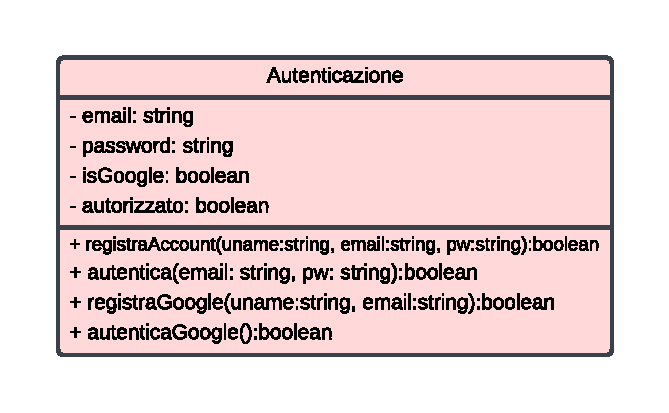
\includegraphics[scale = 0.9]{materiale/class-autenticazione.pdf}
\caption{Definnizione della classe \texttt{Autenticazione}}
\label{autenticaz}
\end{figure}


\subsection{Recupero dell'account}
Nel Diagramma dei Componenti viene individuata la \textit{Pagina di Recupero},
che offre supporto agli utenti registrati, con sistema di credenziali interne,
che hanno dimenticato la password e che intendono recuperare l'account.
Nel Diagramma di Contesto, il servizio di posta elettronica rientra nello
scambio di informazioni necessario per la procedura di recupero. Per
questi motivi viene definita la classe \texttt{RecuperoPwUtente} (Figura \ref{recupero}), che
raccoglie attributi e metodi necessari per effettuare il recupero,
interagendo tra l'altro con il servizio di posta elettronica.

\begin{itemize}
    \item \texttt{email}: l'indirizzo email di recupero viene memorizzato
    per conservarlo durante tutta la procedura di recupero.

    \item \texttt{mandaEmailRecupero}: il messaggio di recupero viene inviato
    all'indirizzo specificato. Questo metodo rappresenta la richieste di
    invio da parte del sistema nei confronti del servizio di posta.

    \item \texttt{cambiaPassword}: la nuova password inserita dall'utente
    viene aggiornata nel suo account. Come rappresentato dal Diagramma dei
    Componenti, questa è la realizzazione dell'interfaccia fornita al
    database. Questa operazione può essere effettuata solo su un account
    già registrato e quindi esistente, come mostrato dal tipo del secondo
    parametro richiesto (\texttt{UtenteAutenticato}).
\end{itemize}
Questa classe è coinvolta in una associazione con \texttt{User}, la quale
richiede il recupero facendo riferimento ad una sola istanza di
\texttt{RecuperoPwUtente}, mentre quest'ultima, a sua volta, si occupa
delle operazioni di recupero per conto di un utente solo.

\begin{figure}[H]
\centering
\hspace*{-1.5cm}
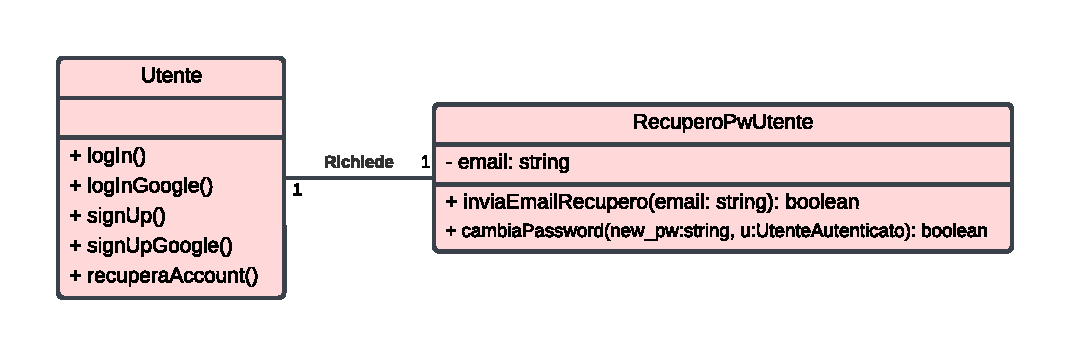
\includegraphics[scale = 0.8]{materiale/class-recupero.pdf}
\caption{Specifica architetturale del componente \textit{Pagina di Recupero} con la classe \texttt{RecuperoPwUtente}}
\label{recupero}
\end{figure}



\newpage
\subsection{Catalogo}
Il \textit{Catalogo} presente nel Diagramma dei Componenti è rappresentato in
Figura \ref{catalog} sotto forma di due classi: \texttt{UtenteAmministratore}, descritto insieme
alle altre categorie di utenti, e \texttt{Catalogo}. Tale scelta architetturale
è giustificata dall'esigenza di identificare chiaramente il ruolo dell'utente
amministratore, mantenendo dunque una definizione dei livelli di accesso
coerente con quella dei documenti precedenti, oltre alla volontà di ridurre il
carico di informazione della classe \texttt{Catalogo} rendendo il rispettivo
componente del diagramma più modulare e non monolitico.
\begin{itemize}
    \item \texttt{problemi[1...*]}: questo attributo indica che il catalogo
    consiste in una lista di almeno un problema (si veda la prossima sezione
    per i dettagli sui problemi).
    
    \item \texttt{cercaPerTag}:
    \item \texttt{cercaPerNome}:
    \item \texttt{filtraDifficolta}: questo metodo consente di filtrare i
    problemi mostrati nel catalogo sulla base della loro difficoltà. Il
    tipo enumerato \texttt{Difficulty} in Figura \ref{catalog}
    raccoglie i livelli esistenti.

    \item \texttt{mostraHint}: sulla base del metodo selezionato, il metodo
    interagisce con YouTube per visualizzare il video-suggerimento.

    \item \texttt{mostraPreferiti}:
    \item \texttt{mostraStato}:
    \item \texttt{mostraProblema}:
\end{itemize}

\begin{figure}[H]
\centering
%\hspace*{-1.5cm}
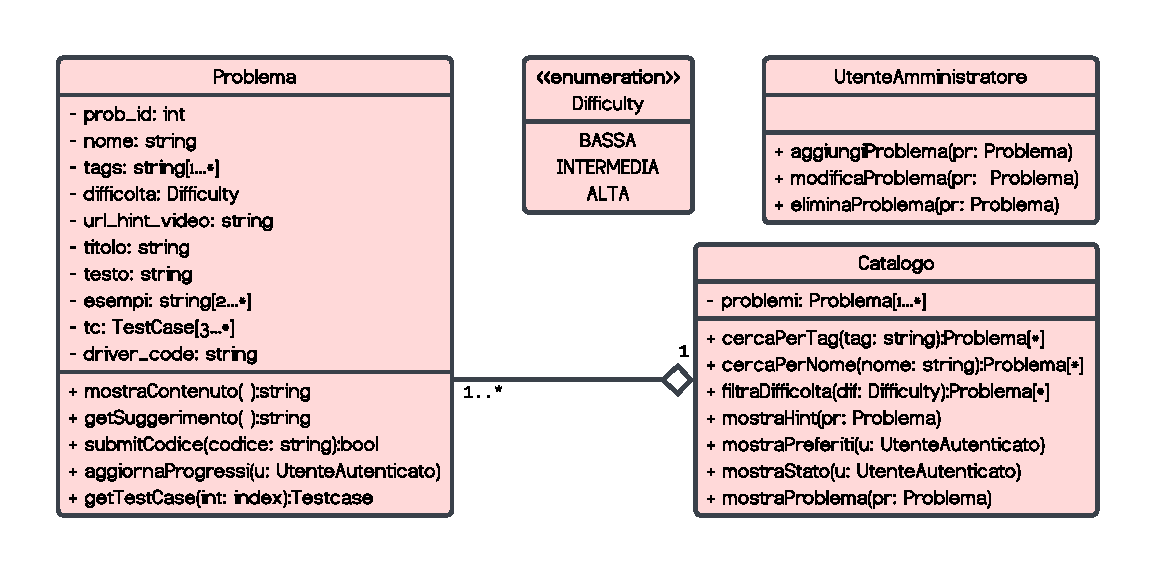
\includegraphics[scale = 0.7]{materiale/class-catalogo.pdf}
\caption{Specifica architetturale del componente \textit{Catalogo} con la classe \texttt{Catalogo}}
\label{catalog}
\end{figure}



\newpage
\subsection{Problemi ed Esercitazione}
La Figura \ref{esercitaz} illustra le classi che costituiscono il componente
\textit{Pagina di Esercitazione}.

\begin{figure}[H]
\centering
%\hspace*{-1.5cm}
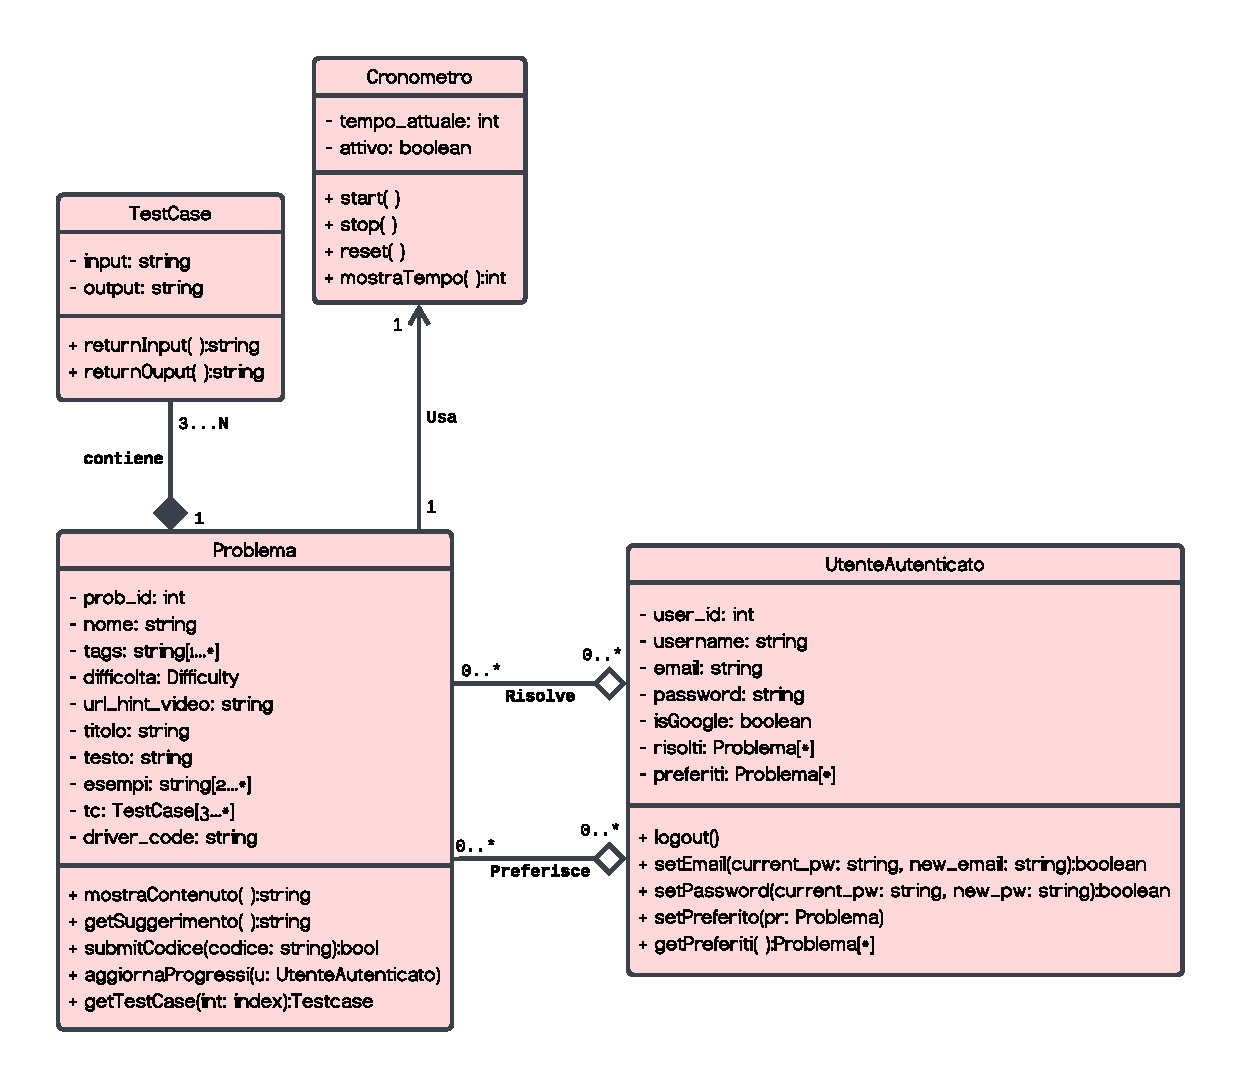
\includegraphics[scale = 0.6]{materiale/class-esercitazione.pdf}
\caption{Specifica architetturale del componente \textit{Catalogo} con la classe \texttt{Catalogo}}
\label{esercitaz}
\end{figure}








\newpage
\section{Specifiche in codice OCL}
Nella sezione che segue viene descritta formalmente la logica prevista
nel comportamento di alcune classi, in relazione alle loro operazioni
possibili. Il codice OCL impiegato consente di esprimere tale logica,
non descrivibile con i soli diagrammi delle classi in UML.















\newpage
\section{Diagramma delle classi con codice OCL}
In Figura \ref{umlocl} è riportato un diagramma che mostra nell'insieme
sia le classi individuate che il relativo codice OCL, definiti nelle
sezioni precedenti.

\begin{figure}[H]
\centering
\hspace*{-2.8cm}
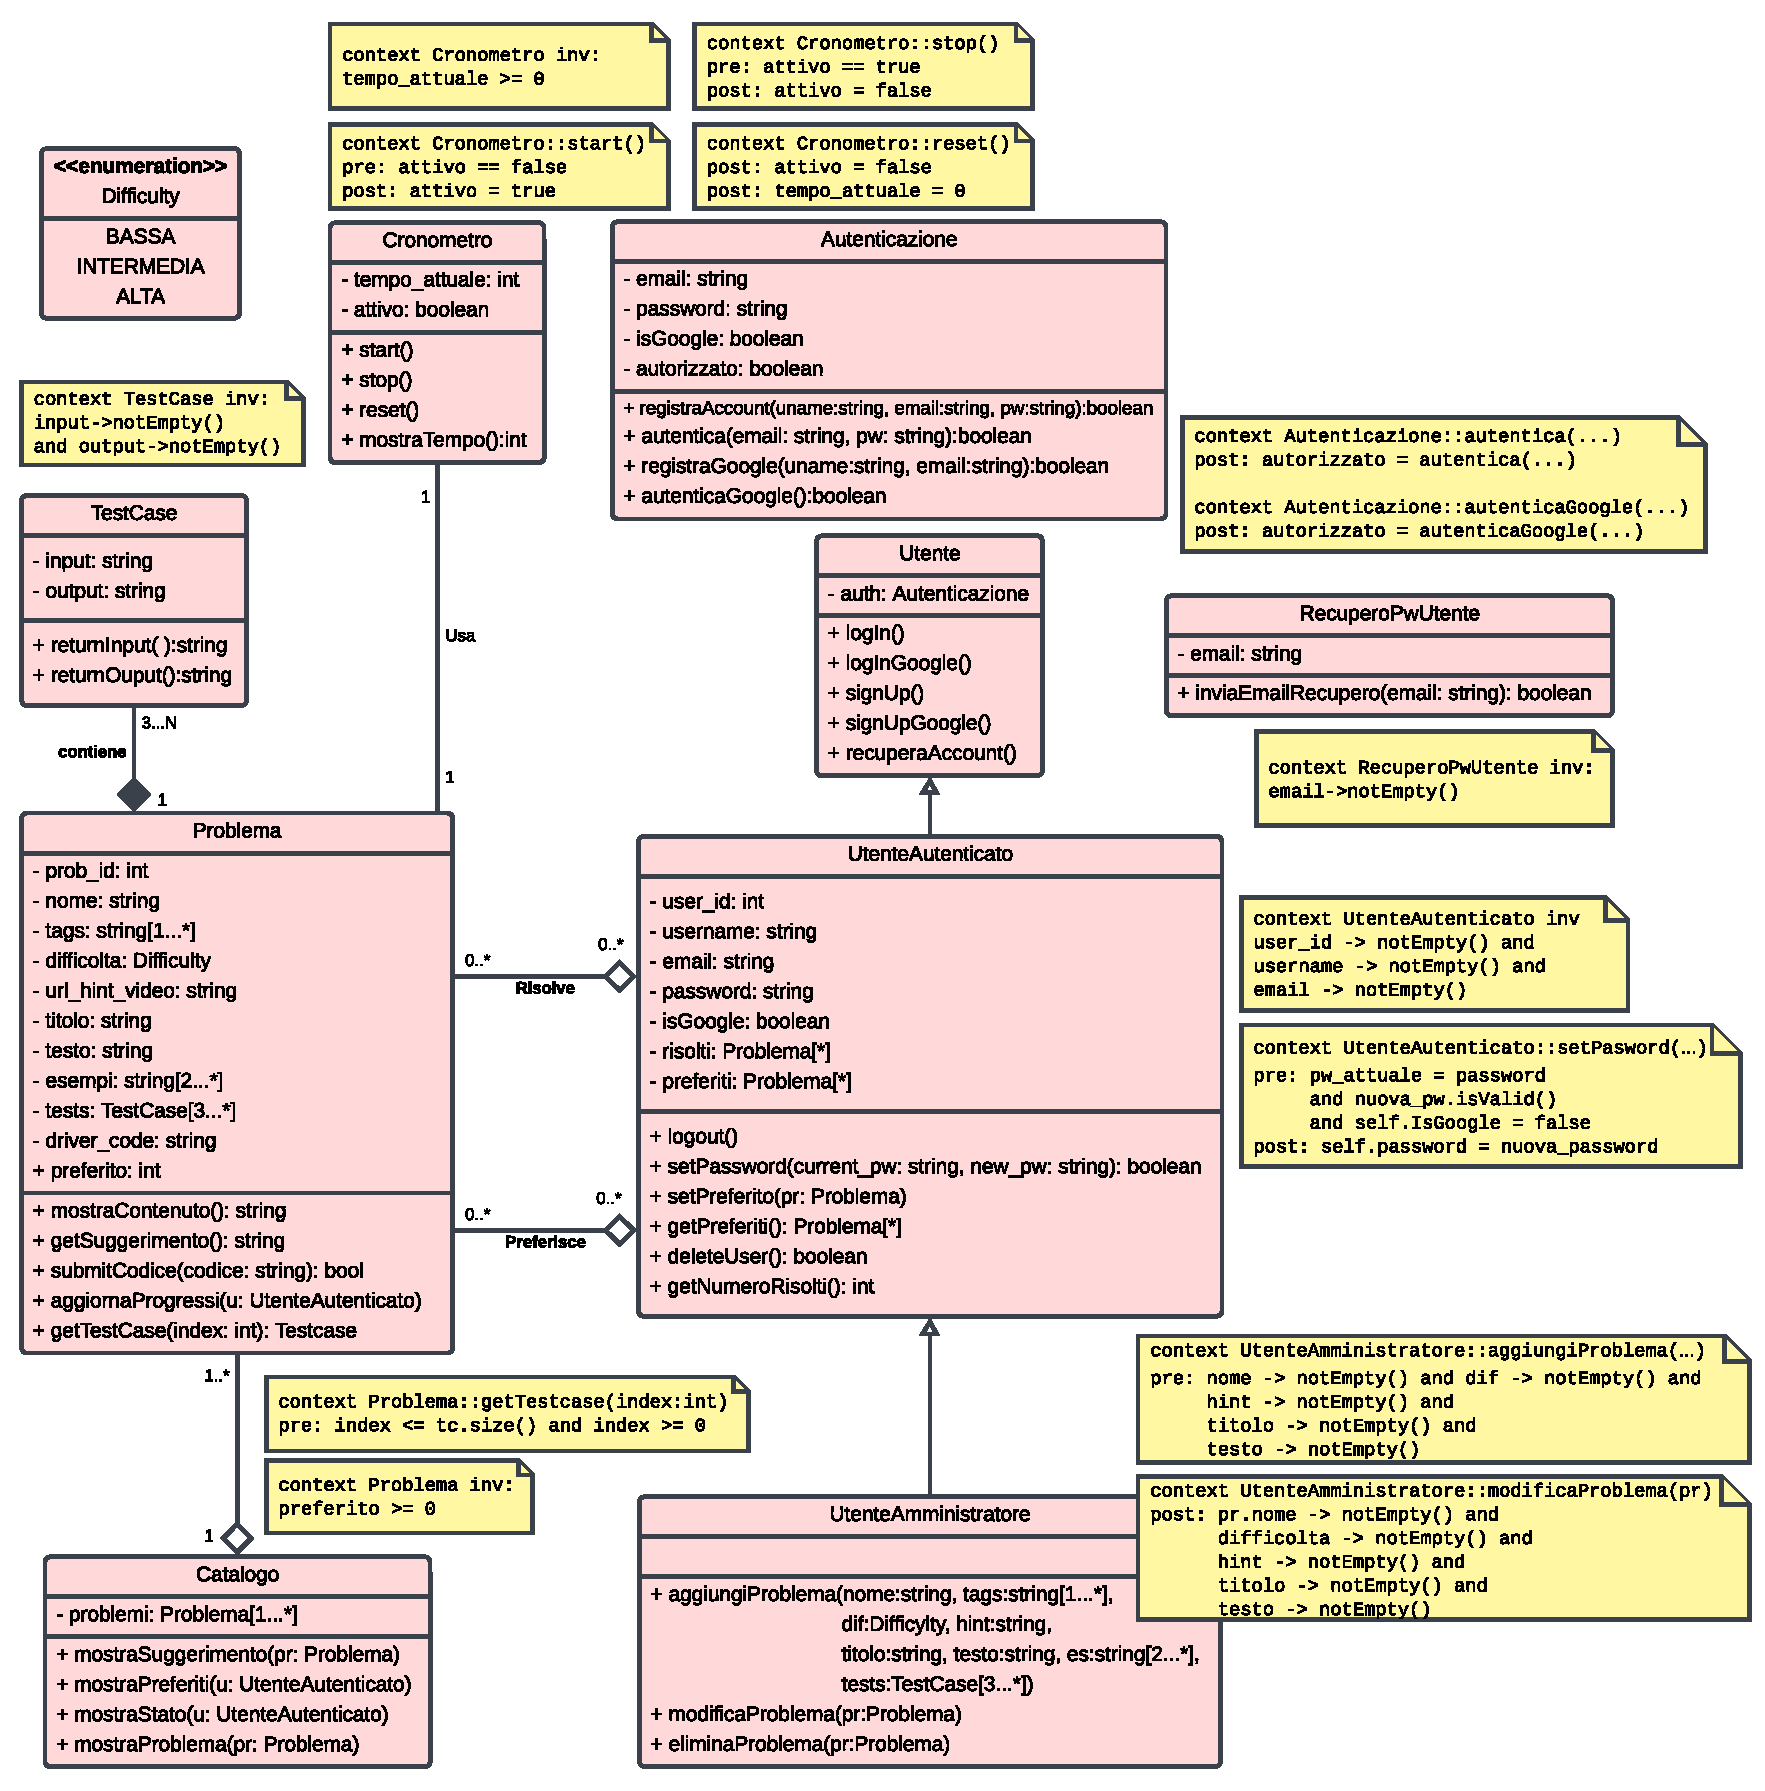
\includegraphics[scale = 0.53]{materiale/classdiagram.pdf}
\caption{Diagramma delle classi arricchito da codice OCL}
\label{umlocl}
\end{figure}

\end{document}